\documentclass{standalone}
\usepackage{tikzducks}
\pagecolor{gray!20!white}
\begin{document}
	
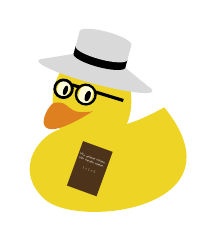
\begin{tikzpicture}
	\duck[glasses,
	bookcolour=black!60!brown,
	book={
			\scalebox{0.14}{
			\parbox{2.5cm}{
			\sffamily
			\centering
			\footnotesize
	    Wir m\"ussen wissen.\\
	    Wir werden wissen.\\[0.4cm]
	    $1+1=2$}}},
	strawhat
	]
\end{tikzpicture}	
	
\end{document}